\documentclass{article}
\usepackage[utf8]{inputenc}
\usepackage[spanish]{babel}
\usepackage{listings}
\usepackage{graphicx}
\graphicspath{ {images/} }
\usepackage{cite}

\begin{document}

\begin{titlepage}
    \begin{center}
        \vspace*{1cm}
            
        \Huge
        \textbf{Taller 1}
            
        \vspace{0.5cm}
        \LARGE
        Calistenia
            
        \vspace{1.5cm}
            
        \textbf{Juan Diego Carrera Quintero}
            
        \vfill
            
        \vspace{0.8cm}
            
        \Large
        Despartamento de Ingeniería Electrónica y Telecomunicaciones\\
        Universidad de Antioquia\\
        Medellín\\
        Marzo de 2021
            
    \end{center}
\end{titlepage}

\tableofcontents
\newpage
\section{Descripción del ejercicio}\label{intro}
Para este ejercicio necesitarás llevar unos objetos desde la posición inicial (Figura \ref{fig:pocision1}) hasta una posición final (Figura \ref{fig:pocision2}) utilizando únicamente una sola mano, para llevar a cabo este ejercicio deberás seguir las siguientes instrucciones; importante no hacer nada que no esté descrito en los pasos, seguirlos exactamente como están escritos.

\section{Ilustraciones}\label{imagenes}

\begin{figure}[h]
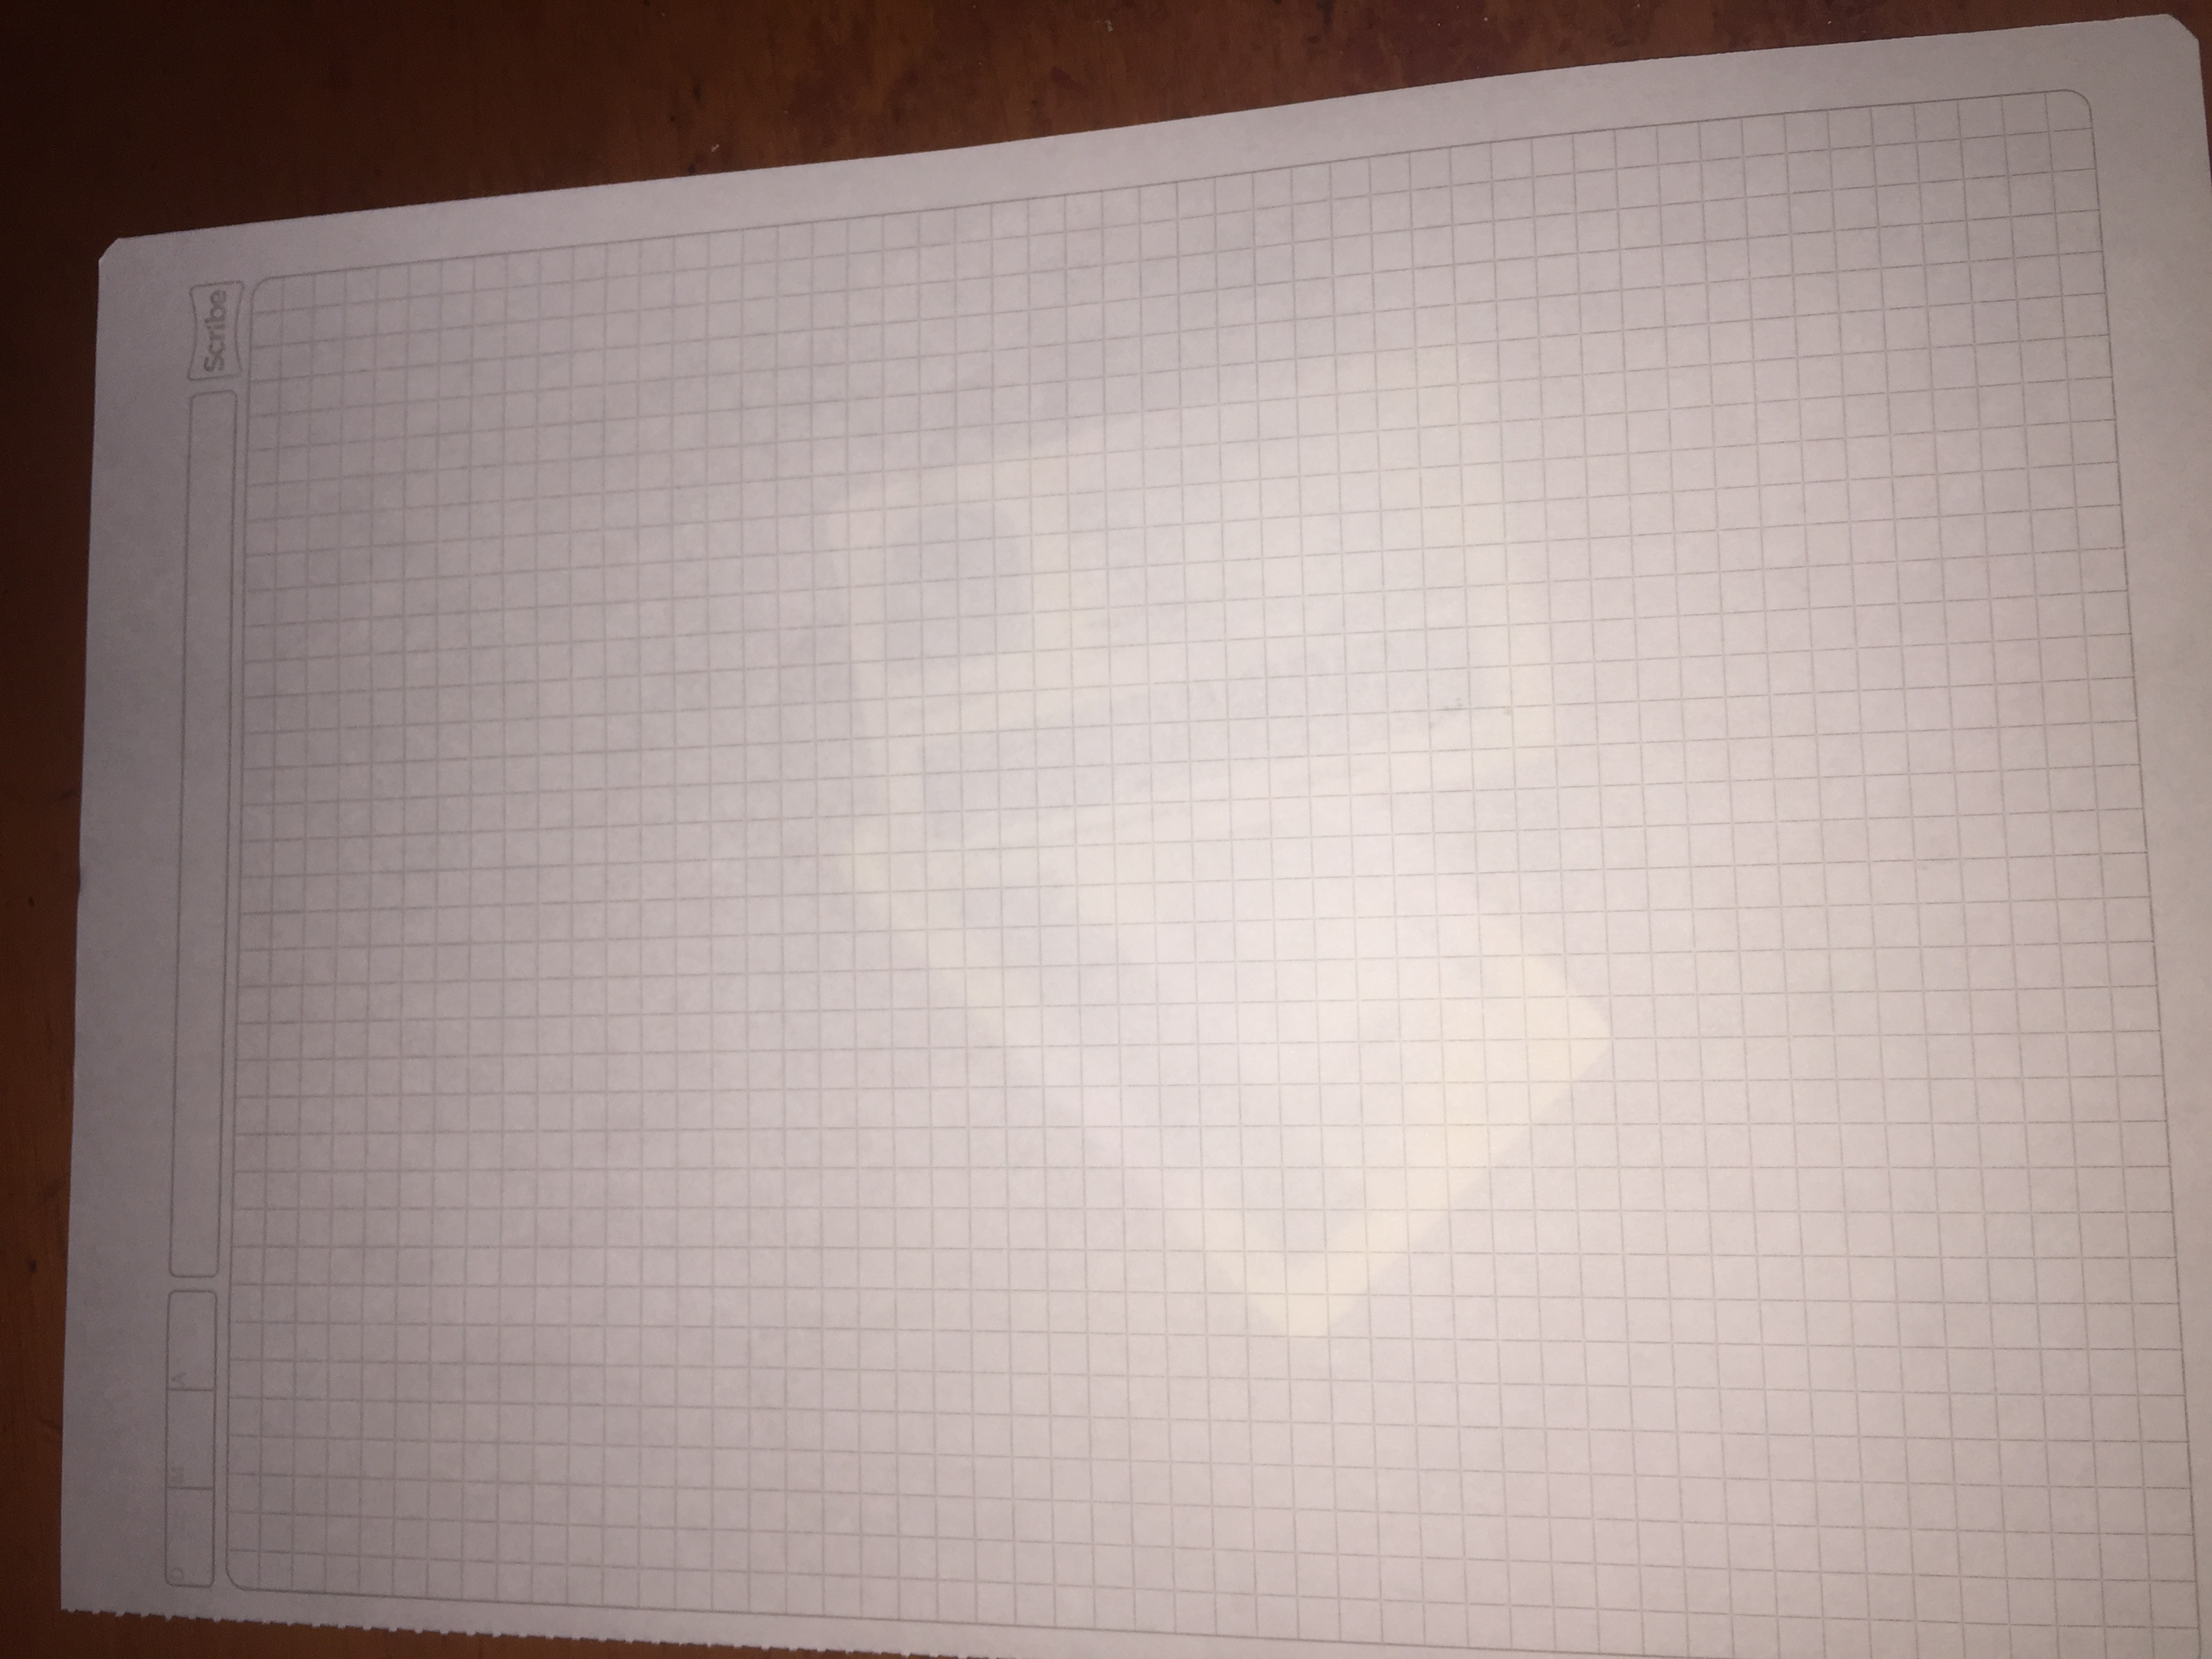
\includegraphics[width=8cm]{posición1.JPG}
\centering
\caption{posición inicial}
\label{fig:pocision1}
\end{figure}

\begin{figure}[h]
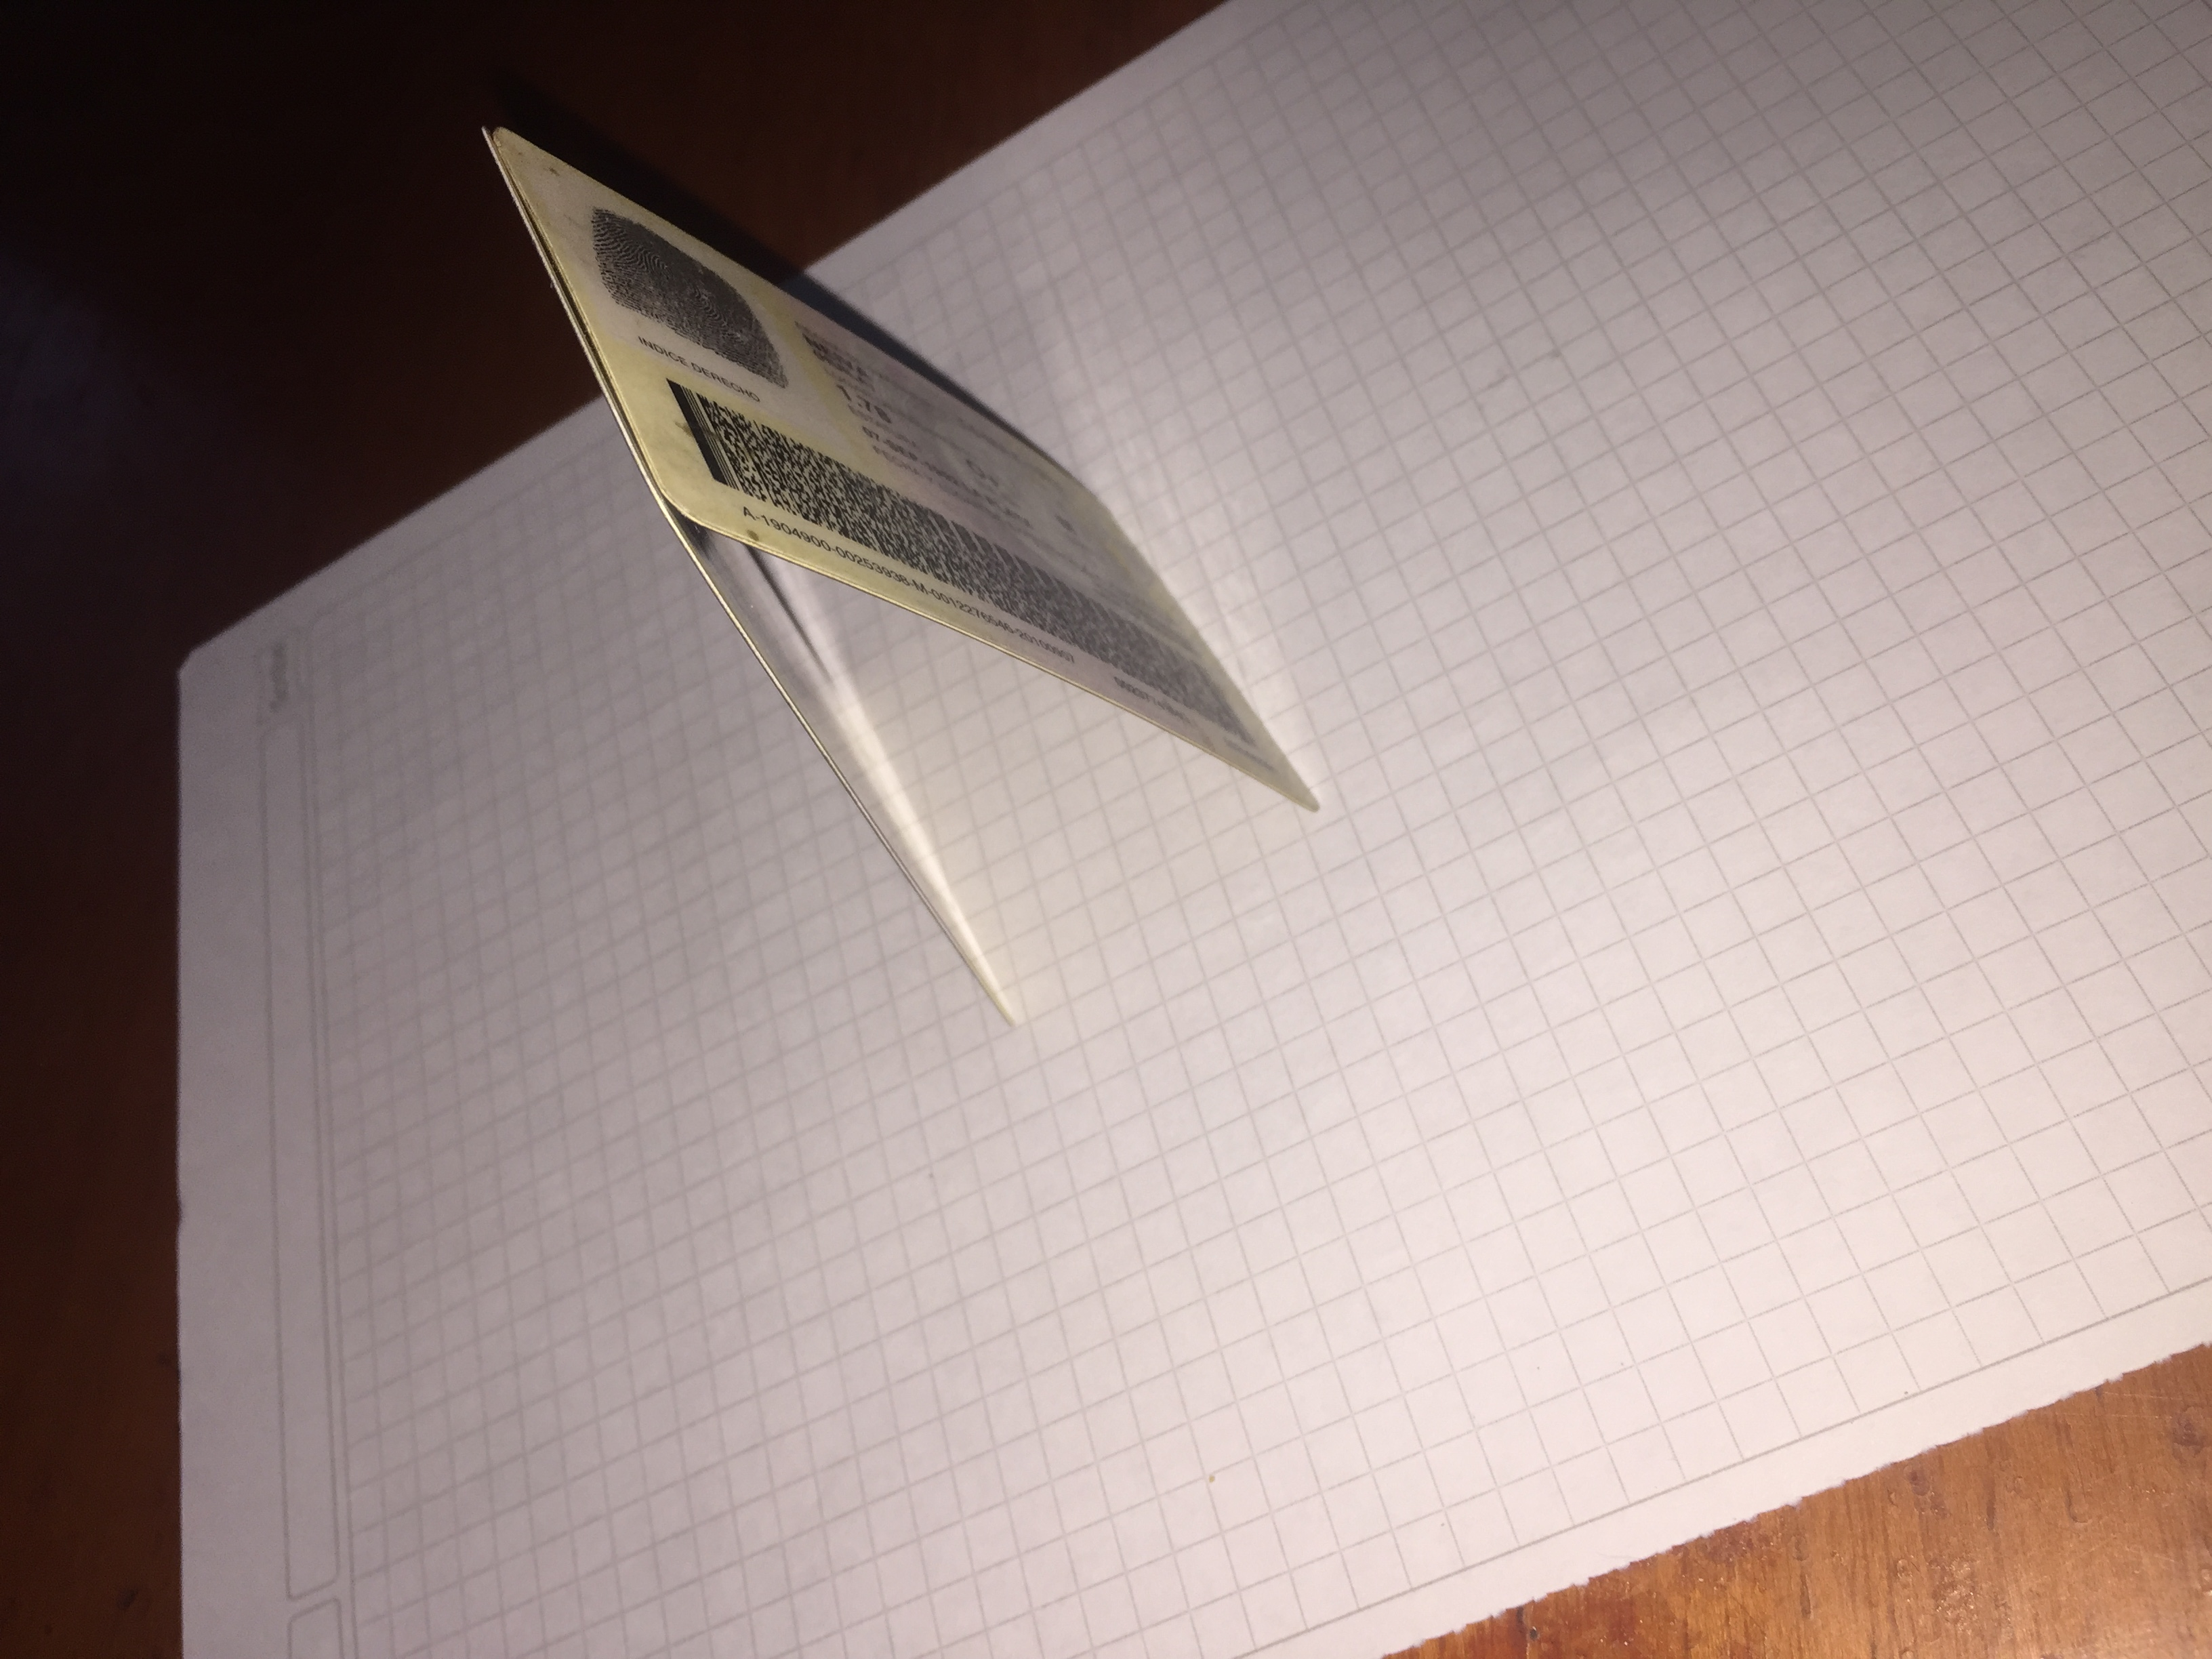
\includegraphics[width=8cm]{posición2.JPG}
\centering
\caption{posición final}
\label{fig:pocision2}
\end{figure}

\section{Pasos} \label{contenido}
Recuerda seguir los pasos tal cual como están escritos.
\begin{enumerate}
    \item Elegir con qué mano quieres trabajar, derecha o izquierda, ya sea tu mano dominante o la que quieras.
    \item Deja tu otra mano a un lado, no podrás hacer uso de esta.
    \item Ahora con la mano con la que vas a trabajar levanta la hoja de papel y ponla a un lado sobre la mesa, dejando a la vista las tarjetas.
    \item Agarra ambas tarjetas y ponlas sobre la hoja.
    \item Con las tarjetas sobre la hoja usa tu mano para alinearlas de tal forma que se vea un solo rectángulo.
    \item Ubica los lados más largos de las tarjetas.
    \item Pon tu dedo pulgar en el lado largo más cercano a ti.
    \item Pon tus dedos medio y anular en el lado largo contrario al que tiene tu dedo pulgar.
    \item Pon tu dedo índice sobre el lado corto que está más cerca de éste.
    \item Con tus cuatro dedos levanta las tarjetas y asegúrate de que estén las dos.
    \item Levanta las tarjetas a una altura de más o menos 5 centímetros sobre la hoja.
    \item Sin soltar las tarjetas ubícalas de manera vertical, con el dedo índice arriba del resto y sostenlas en esa posición.
    \item Baja las tarjetas en la misma posición anterior asegurándote de que las tarjetas y la hoja estén en contacto.
    \item Suelta tus dedos pulgar, medio y anular, de tal forma que las tarjetas estén entre la hoja y tu dedo índice.
    \item Mientras tu dedo índice está sosteniendo ambas tarjetas, con tus dedos pulgar, medio y anular sujeta solo una tarjeta, la que esté más cerca de ellos.
    \item Aun con tu dedo índice sosteniendo ambas tarjetas usa tus otros tres para separar la parte inferior de la tarjeta que están sosteniendo, de tal forma que las dos tarjetas y la hoja hagan forma de triángulo.
    \item Una vez las tarjetas formen un triángulo haz que se mantengan en equilibrio y suéltalas lentamente.
    \item Si las tarjetas no se caen haz finalizado el reto exitosamente.
    \item Si las tarjetas se caen vuelve a repetir el proceso desde el paso 5 o retírate sin completar el reto.

\end{enumerate}

\end{document}